\acresetall

The goal of this thesis is to develop the control for the optical spring
experiment, observe the signature of the optical spring in the transfer
function, and determine the noise level and steps for noise mitigation
in order to remove active feedback at the spring resonance.

In this chapter I will define the sources of noise which we have identified
and describe their impact to the experiment.

We have identified sources of noise and projected their contribution to noise
in the length of the cavity.
We could also choose frequency of the light as a reference, but we choose the
cavity length as this is the natural dimension when talking about a spring,
$F=-kx$.
This "noise budget" is necessary for building the full picture for explaining our
observations.

The \ac{pdh} error signal for the trap cavity is our observation of the length
of the cavity.
With the cavity locked we use the \ac{pdh} signal to infer residual motion of
the cavity.
We calibrate the error signal by measuring the open loop gain and dividing out
the feedback servo and actuation function.

\section{Seismic}
\label{sec:seismic}

Seismic noise in our lab was a bit problematic due to the fact there is a giant
inflatable roof sports dome right next door. The fans required to keep the roof
up create a great deal of seismic noise at specific frequencies.

This causes peaks in our seismic spectrum at frequencies that are integer
multiples of each fans rotational frequency $\Omega_f$.
The frequency at $n_b\Omega_f$, where $n_b$ is the number of blades in the fan,
will likely be the highest since a section of air near the fan will feel an
increase in force as each blade passes by. The seismic noise is plotting along
with noise measured from the two suspensions in figure \ref{fig:seismic}.

Aside from the seismic peaks, the background seismic spectrum was basically as
expected.
The falloff was $1/f^2$ with $\approx 10^{-10} \mathrm{m/\sqrt{Hz}}$ at
$\mathrm{100 Hz}$.
The total rms motion was less than $1\mu \mathrm{m}$ at $\mathrm{100 mHz}$.
With a voltage range of $\pm 10 \mathrm{V}$ at the coil drivers for our
suspensions we can get a position range of about $\pm 68\mathrm{\mu m}$ for
the suspended mass at DC.
This gives us plenty of range to cover the background seismic motion.

\begin{figure}
  \centering
  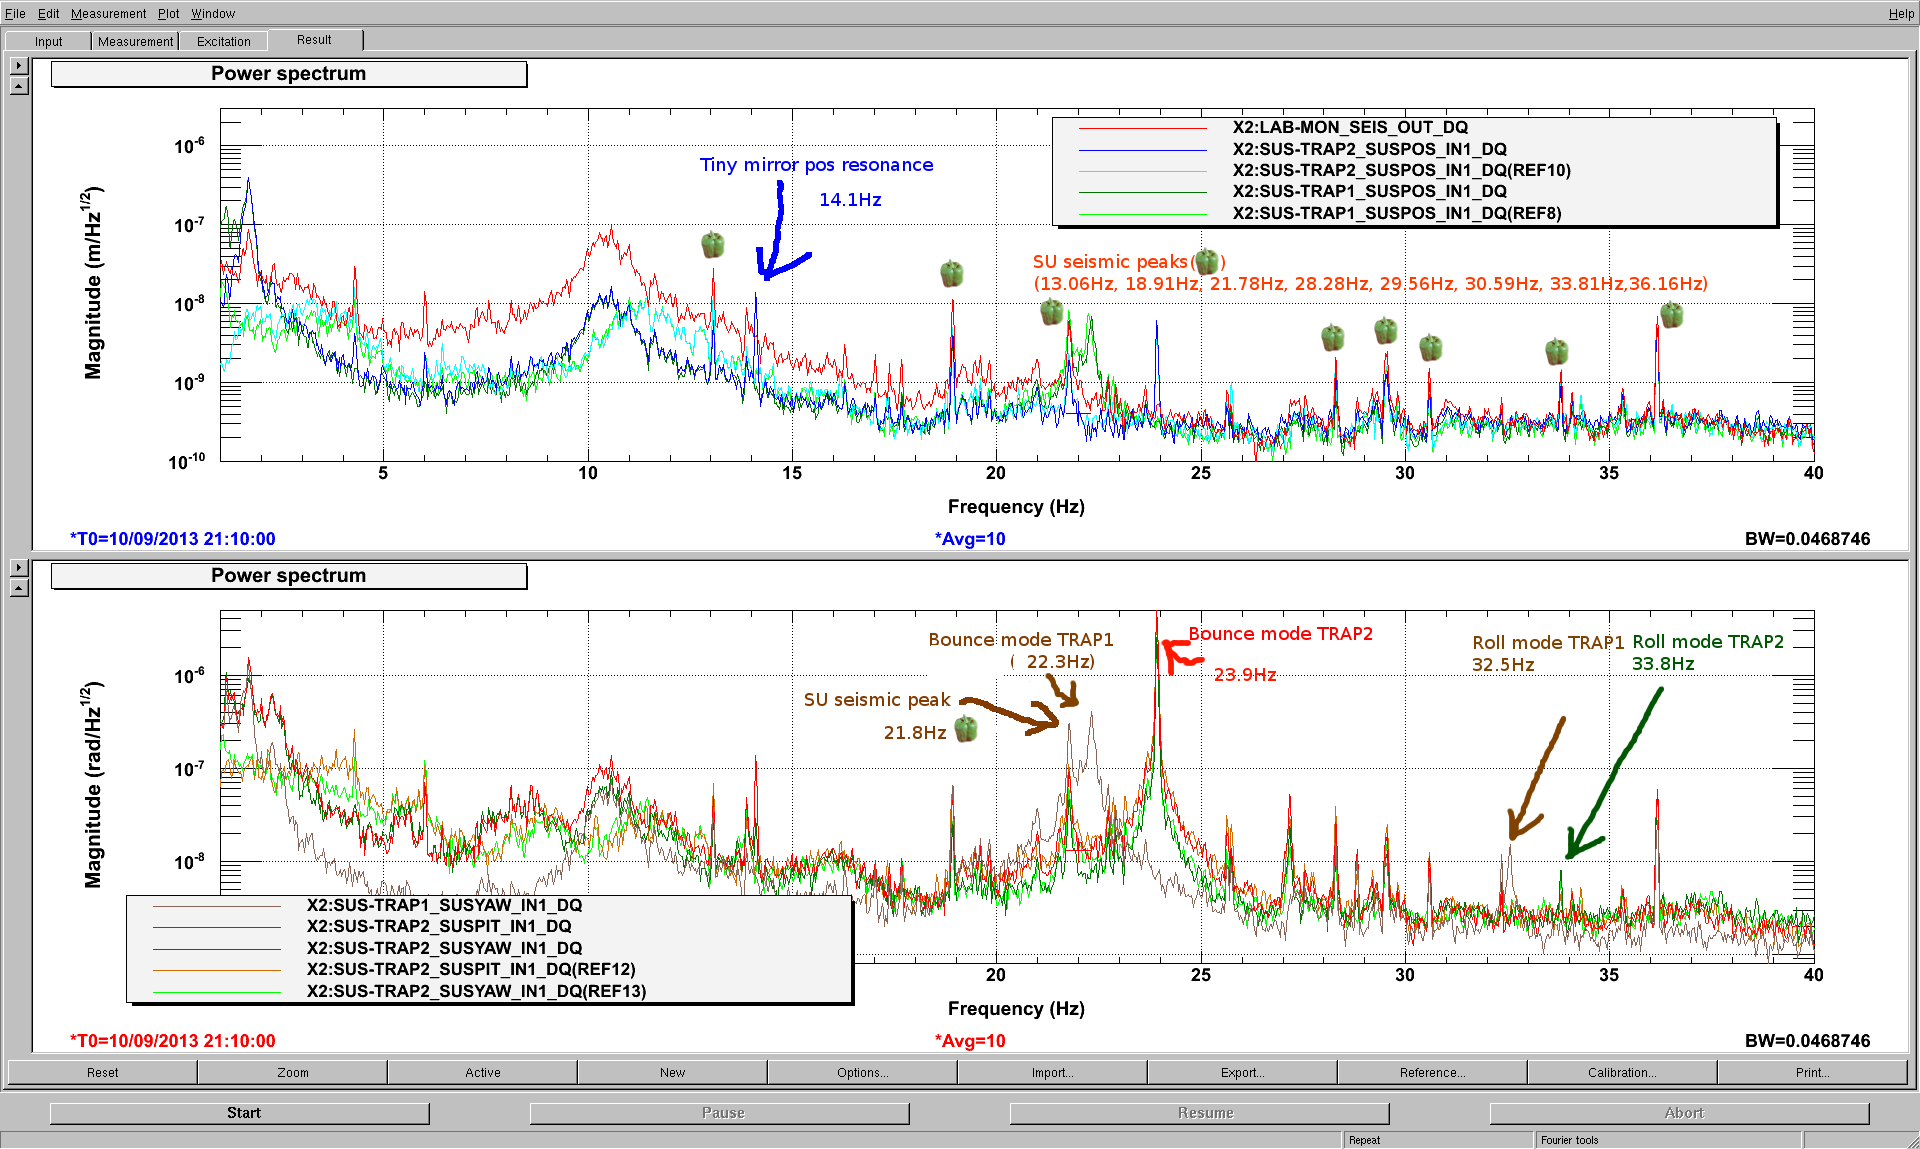
\includegraphics[width=15cm]{./figures/modehunting.png}
  \caption[Seismic Noise Spectrum]{
    This shows the spectrum of the seismic noise in our lab taken with a
    seismometer located on table 2.
    The peppers represent peaks in the seismic background.
    This spectrum was taken with the first payload assembly
    suspended from our small optic suspension
    before installing blade springs for vertical isolation.
    We needed to move the bounce mode frequency down in order to not excite
    it with the background seismic peaks.
    The suspension upgrade took place concurrently with the payload upgrade
    discussed in section \ref{sec:highQsus}.
    }
  \label{fig:seismic}
\end{figure}


%\begin{figure}
%  \centering
%  \tikzsetnextfilename{seismic}
%  \begin{tikzpicture}
%  \begin{loglogaxis}[
%    name=plot1,
%    height=7cm,
%    width=14cm,
%    ylabel={$\mathrm{m}/\sqrt{\mathrm{Hz}}$},
%    xlabel={Frequency $(\mathrm{Hz})$},
%    grid=both,
%  ]
%    \addplot[red,very thick,domain=1:1000] {1/(x*x-1)};
%  \end{loglogaxis}
%  \end{tikzpicture}
%  \caption[Lab Seismic Spectrum]{This is the seismic spectrum we have in the lab.
%    }
%  \label{fig:seismic}
%\end{figure}

\section{Thermal}

Thermal noise is the random aggregate fluctuations of an object due to the
random motion of the constituent particles.
The spectral density of this motion is dependant on the temperature and the
dissipation of the material.
The random motion in a dimension of interest also depends on the geometry of
the system.

These motions are tiny and only really affect us in a cavity where we rely on
the constructive interference of the micron wavelength light.
So, we look closely at the materials in direct contact with the mirrors.

Specifically, we identify the payload suspension attachment to the small
mirror, the aluminum disk within which the large mirror is imbedded, and the
layers of the high reflective coatings.

Thermal noise will also affect us indirectly if we use another cavity for
reference.
The \ac{fss} will not be able to suppress the frequency noise below the
thermal noise from the mirrors of the reference cavity.
This thermal noise is part of the sensing noise for the servo and thus gets
imprinted on the laser frequency which will account for detuning noise of
the cavity.

If we were to implement the \ac{fss} we would need to account for the
reference cavity's thermal noise as well.
% This would be the case for us if we were to implement the \ac{fss} described
% in section \ref{sec:fss}.
We estimate these noise effects as well in order to quantify the possible
improvements gained by the implementation of this system.

Thermal noise from the reference cavity consists of the same coating thermal
for the trap cavity and thermal noise from the glue used to attach the
mirrors on the ends of the fused silica spacer.

\subsection{Derivation of Payload Suspension Thermal Noise}

We derive the thermal noise of a system using the fluctuation-dissipation
theorem which describes the relationship between the fluctuation of a system
and its dissipation.
The starting point for our thermal noise calculations
is the Callen form of the theorem \cite{Saulson,Callen}.

This calculation requires us to know the dynamics of the system.

The \ac{psd} of the thermal noise is defined,
\begin{align}
S_{xx}(\omega) =& \frac{4 k_B T}{\omega^2} \Re (Y(\omega)) \\
    =& \frac{4 k_B T}{\omega^2} \Re (Y(\omega))
\end{align}
For a system with velocity damping($b$), $F_{\mathrm{ext}} = m\ddot{x} + b\dot{x} + kx$,
we can rewrite the \ac{psd} as,
\begin{align}
S_{xx}(\omega) =& \frac{4 k_B T}{\omega^2} \Re (Y(\omega)) \\
    =& \frac{4 k_B T b / \omega^2}{ b^2 + (m \omega - k/\omega)^2}
\end{align}
Notice that as the damping coefficient goes to zero, this function becomes a
delta function at the resonant frequency, $\omega_0 = \sqrt{k/m}$.

That works for something like gas damping. However, we are more interested in
the thermal noise due to internal damping where the damping is essentially
absorbed into the spring coefficient making it complex. This changes the
dependence of the \ac{psd} on $\omega$. Taking this new form of damping,
$F_{\mathrm{ext}} = m\ddot{x} + k(1+i\phi)x$, where $\phi$ is called the
loss angle (for small values of $\phi$) we can write the PSD as,
\begin{align}
S_{xx}(\omega) = & \frac{4 k_B T k \phi / \omega}{(k \phi)^2 +
    (m \omega^2 - k)^2}
\end{align}
In this case we still have the peak at the resonant frequency, however the form
of the noise is different above and below the resonant frequency.

\begin{figure}
\centering
  \tikzsetnextfilename{tnoisesketch}
  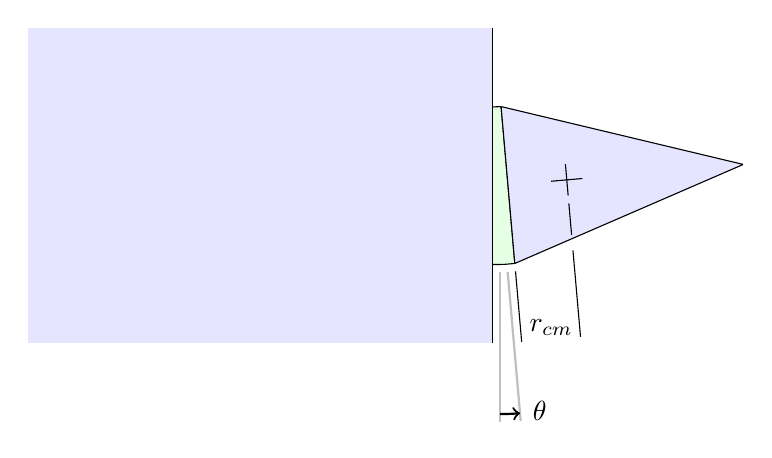
\begin{tikzpicture}
    \draw[gray!50,thick] (0,-1.1) -- (0,-3);
    \draw[gray!50,thick] (275:1.1) -- (275:3);
    \draw[black,thick,->] (0,-2.9) arc (270:275:2.9);
    \node (angle) at (280:2.9) {$\theta$};
    \filldraw[rounded corners=0.1mm,fill=green!10] (-0.1,1) -- (-0.1,-1) -- ++(0.1,0)
      arc (270:275:1) -- ++(5:0.1) -- ++(95:2) -- cycle;
    \fill[fill=blue!10] (-0.1,2) rectangle (-6,-2);
%    \shade[top color=white,bottom color=blue!10] (-0.1,2) rectangle (-6,3);
    \draw (-0.1,2) -- (-0.1,-2);
    \filldraw[rounded corners=0.1mm,fill=blue!10,rotate=5] (0.1,1) -- ++(0,-2)
      -- (3.1,0) -- cycle;
    \draw[rotate=5] (0.1,-1.1) -- (0.1,-2);
    \draw[rotate=5] (0.85,-0.9) -- (0.85,-2);
    \draw[rotate=5] (0.85,-0.3) -- (0.85,-0.7);
    \draw[rotate=5] (0.85,-0.2) -- (0.85,0.2);
    \draw[rotate=5] (0.65,0) -- (1.05,0);
    \node (rcm) at (0.65,-1.8) {$r_{cm}$};
  \end{tikzpicture}
  \caption[Sketch of Thermal Noise Calculation]{
    This shows the setup for the thermal noise derivations starting with
    equations \ref{eq:fullT}.
    The fiber is not included in the calculation for this.
    }
  \label{fig:tnoisesketch}
\end{figure}

Now we will derive the thermal noise for our small mirror assembly. We are
concerned with thermal noise due to the epoxy used to glue the fibers to the
mass. We start with the Lagrangian to get the dynamics of the system and
compute the admittance.
\begin{align}
\begin{split} \label{eq:fullT}
T &= \frac{1}{2} M \dot{x}^2 +
    \frac{1}{2}I_M \left( \dot{\eta_1}^2 + \dot{\eta_2}^2 \right) \\
    &\quad + \frac{1}{2} m \left(
    \dot{x} + r_M \dot{\eta_1}
    + r_{\mathrm{cm}} \dot{\theta_1} \right)^2 \\
    &\quad + \frac{1}{4} m \left(
    2 \dot{x} - r_M \left(
    \dot{\eta_1}
    + \sqrt{3} \dot{\eta_2} \right)
    + 2r_{\mathrm{cm}} \dot{\theta_2} \right)^2 \\
    &\quad + \frac{1}{4} m \left(
    2 \dot{x} - r_M \left(
    \dot{\eta_1}
    - \sqrt{3} \dot{\eta_2} \right)
    + 2r_{\mathrm{cm}} \dot{\theta_3} \right)^2 \\
    &\quad + \frac{1}{2} I_m \left[
    \left( \dot{\theta_1} + \dot{\eta_1} \right)^2
    + \frac{1}{2} \left( 2\dot{\theta_2} - \dot{\eta_1} - \sqrt{3} \dot{\eta_2} \right)^2
    + \frac{1}{2} \left( 2\dot{\theta_3} - \dot{\eta_1} + \sqrt{3} \dot{\eta_2} \right)^2
    \right]
\end{split} \\
\label{eq:fullV}
V &= \frac{E l_y l_x^3}{8t} \left( \theta_1^2 + \theta_2^2 + \theta_3^2 \right)
\end{align}
Where $x$ is the position of the mirror, $\eta_1$ and $\eta_2$ are the pitch and yaw
of the mirror, and $\theta_i$ are the angles of each fiber attachment nub with
respect to the mirror.

The equations of motion become quite complex, so we simplify the system by only
looking at the contribution from the longitudinal mode. The effects of the pitch
and yaw modes should not contribute at first order for a perfectly aligned
system, so we can simplify \eqref{eq:fullT} and \eqref{eq:fullV} by setting
$\dot{\eta_1}=\dot{\eta_2}=\dot{\eta_3}=0$ and
$\theta_1=\theta_2=\theta_3=\theta$.
The equations then become
\begin{align}
T &= \frac{1}{2} M\dot{x}^2
    + \frac{3}{2} m\left(\dot{x}+r_{\mathrm{cm}}\dot{\theta} \right)^2
    + \frac{3}{2} I\dot{\theta}^2 \\
V &= \frac{E l_y l_x^3}{8t}\theta^2 
\end{align}
making some substitutions,
\begin{align}
m_t &= M+3m \, , \\
I_t &= 3 \left( mr_{\mathrm{cm}}^2+I \right) \, , \\
K &= \frac{E l_y l_x^3}{4t} \, ,
\end{align}
the Lagrangian becomes,
\begin{align}
\frac{1}{2} \left( m_t \dot{x}^2 +6mr_{\mathrm{cm}}\dot{x}\dot{\theta}
+ I_t\dot{\theta}^2 -K\theta^2 \right) \, .
\end{align}
We can then find the equations of motion with an external force in
the $x$ direction,
\begin{align}
F_{\mathrm{ext}} &= \frac{d}{dt}\frac{\partial L}{\partial \dot{x}}
  - \frac{\partial L}{\partial x} \,.
\end{align}
The two equations of motion become,
\begin{align}
F_{\mathrm{ext}} &= m_t \ddot{x} + 3mr_{\mathrm{cm}}\ddot{\theta} \\
0 &= 3mr_{\mathrm{cm}}\ddot{x} + I_t\ddot{\theta} + K\theta \, .
\end{align}
We can then solve for the impedence in the frequency domain,
\begin{align}
Z = \frac{F_{\mathrm{ext}}}{i\omega x} &= m_t i\omega
  + 3mr_{\mathrm{cm}}i\omega \frac{\theta}{x} \,,
\end{align}
where, from the second equation,
\begin{align}
\frac{\theta}{x} &= \frac{3mr_{\mathrm{cm}}\omega^2}{K-I_t\omega^2} \,.
\end{align}
We need the real part of the admittance, $Y=1/Z$.
\begin{align}
Y &= \frac{iI_t\omega^2-iK}{\omega m_t(K-I_t\omega^2) + (3mr_{\mathrm{cm}})^2\omega^3}
\end{align}
The real part of $Y$ is then,
\begin{equation}
\frac{K_0 \phi \omega (3mr_{\mathrm{cm}})^2}{ \left(
  m_tK_0 + \omega^2 \left( (3mr_{\mathrm{cm}})^2 -m_tI_t \right) \right)^2
  + (m_tK_0 \phi)^2 }
\end{equation}
And the thermal noise in the $x$ direction is (we have taken $\phi$ to be small),
\begin{equation}
S_{xx}(\omega) = \frac{4k_BT}{\omega} \left[
  \frac{K_0\phi (3mr_{\mathrm{cm}})^2}{\left( m_tK_0 + \omega^2 \left( (3mr_{\mathrm{cm}})^2 -m_tI_t \right)
  \right)^2 }
  \right] \label{eq:tnoisesusfull}
\end{equation}

When $\omega$ is below the resonant frequency,
\begin{align}
S_{xx}(\omega) &= \frac{4k_BT}{m_t^2 \omega}
  \frac{\phi(3mr_{\mathrm{cm}})^2}{K_0} \label{eq:generalmassgluenoise} \\
S_{xx}(\omega) &= \frac{16k_BT\phi t(3mr_{\mathrm{cm}})^2}{m_t^2 \omega El_yl_x^3}
\end{align}
It is desirable to make the nubs much smaller than the mirror.
So, we can simplify the equation to,
\begin{align}
S_{xx}(\omega) &= \frac{36k_BT\phi t l_yl_z^4\rho^2}{M^2\omega El_x} \,.
\end{align}
Now, it is obvious that we want to make the nubs so that the center of mass is
close to the mirror, the thickness of the glue is small, and the glue area is
large in the dimension along the axis of the mirror.

For our situation we have actually arrived at a cone shaped nub which provides
for a large base and a short $r_{\mathrm{cm}}$. Going back to eq.
\eqref{eq:generalmassgluenoise} we make the approximations to get
\begin{align}
S_{xx}(\omega) &= \frac{4k_BT\phi(3mr_{\mathrm{cm}})^2}{M^2 \omega K_0}
\end{align}
The mass of a cone is $\frac{1}{3} \pi R^2 l_z \rho$, $r_{\mathrm{cm}}$ is
$\frac{1}{4} l_z$, and $K_0 = \frac{3\pi ER^4}{4t}$.
\begin{align}
S_{xx}(\omega) &= \frac{k_BT\phi \pi t l_z^4\rho^2}{3M^2 \omega E}
\end{align}
The noise is independent of the radius of the base of the cone, but depends
heavily on the length of the cone. The expressions for $K_0$ assume that
$t$ is large compared to $\frac{R^2}{2R_m}$. Figure \ref{fig:tnoisec}
depicts the \ac{asd} of this epoxy thermal noise contribution to the cavity
length noise.

\begin{figure}
  \tikzsetnextfilename{tnoisecone}
  \begin{tikzpicture}
  \begin{loglogaxis}[
    height=7cm,
    xlabel={Frequency $\left[ \mathrm{Hz} \right]$},
    ylabel={Thermal Noise $\left[ m/\sqrt{\mathrm{Hz}} \right]$},
    grid=minor,
  ]
  \addplot[red,thick] table {python/tnoisecone.dat};
  \end{loglogaxis}
  \end{tikzpicture}
  \caption[Epoxy Thermal Noise Contribution to Trap Length]{This is a plot
    of the thermal noise from the epoxy used to glue the small conical nubs
    for the fiber suspension. This includes the resonance which comes from
    the full expression in \eqref{eq:tnoisesusfull}.}
  \label{fig:tnoisec}
\end{figure}

\subsection{Other Thermal Noise Sources}

As mentioned above, we have several sources of thermal noise to consider.
The sources fall into two basic categories: elastic deformation of an object
and bending at a glue joint.

I have presented the derivation of thermal noise from the glue joints attached to
the payload mirror.
The glue joints for the reference cavity mirrors are done in a similar way,
however the geometry is much simpler.
The equations of motion used were simply from the longitudinal compression of the
glue which attaches the mirror to the spacer.

The reference cavity was glued using 4 spots of the Optocast 3553 per mirror.
The mirrors are one inch in diameter with a radius of curvature of $0.5m$
mounted to a spacer which has a 0.5 inch hole drilled through the middle.
Centering the mirror over the 0.5 inch hole, there is at most a distance of
$120 \mu\mathrm{m}$ from the curved surface of the mirror to the flat end
of the spacer.
I have used a value of $50 \mu\mathrm{m}$ for the thickness of the glue spots.

Parameters for glue used in thermal noise modelling are provided in table
\ref{tab:epoxyparams}.


\begin{table}
  \begin{center}
    \small
    \begin{tabular}{|l|l|l|}
      \hline
      Parameter & Symbol & Value \\
      \hline
      \hline
      Young's Modulus & $E_0$ & 3.378 GPa \\
      \hline
      Density & $\rho$ & 1118 $\mathrm{kg/m^3}$ \\
      \hline
      Loss Angle & $\phi$ & 0.03 \\
      \hline
    \end{tabular}
  \end{center}
  \caption[Epoxy Parameters]{
      parameters of the OptoCast 3553 epoxy resin.
      All parameters were taken from the data sheet except for the loss angle.
      The loss angle $\phi$ has not been measured for this material,
      so a fairly conservative value was assumed.
      }
  \label{tab:epoxyparams}
\end{table}

The other category of thermal noise source that I mentioned comes from the
elastic deformation of an object.
The method chosen for this calculation comes from Levin \cite{PhysRevD.57.659}.
This method is derived from the same form of the fluctuation dissipation therom
as above, except that now, we compute the non-homogeneous deformation of
an object where the deformation has a gaussian profile of the same diameter
as the beam spot.

In the case of the coating thermal noise we use a direct application of the
method presented by Levin.

There is one additional source which I place in the same non-homgeneous
deformation category.
That is the deformation of the aluminum disk which the large mirror is
attached to.
The mirror was attached by thermally expanding the aluminum and allowing it to
cool around the large mirror.
This gives a pretty solid attachment and we expect that the dominant thermal
noise from this mount will come from the non-homogenous deformation of the
aluminum itself.
For this calculation we simply apply the same calculation as we do for the
coating to the aluminum disk with a "beam spot" diameter equal to the
diameter of the large mirror.
This will be correct up to some small geometric correction.



These additional noise sources are presented in figure \ref{fig:thermalnoises}.
The total thermal noise contribution is quite low.
With the fiber suspension design, the dominant thermal noise source is actually
from the coatings.

\begin{figure}
  \tikzsetnextfilename{thermalnoises}
  \begin{tikzpicture}
  \begin{loglogaxis}[
    height=8cm,
    xlabel={Frequency $\left[ \mathrm{Hz} \right]$},
    ylabel={Thermal Noise $\left[ m/\sqrt{\mathrm{Hz}} \right]$},
    xmin=10,
    xmax=1000000,
    ymin=0.000000000000000000001,
    legend cell align=left,
    legend style={legend pos=south west,font=\footnotesize},
    grid=minor,
    ]
    \addplot[blue!90!black,very thick] table[x index=0,y index=1]
      {./matlab_traces/thermalnoises.dat};
    \addplot[green!90!black,very thick] table[x index=0,y index=2]
      {./matlab_traces/thermalnoises.dat};
    \addplot[red!90!black,very thick] table[x index=0,y index=3]
      {./matlab_traces/thermalnoises.dat};
    \addplot[yellow!90!black,very thick] table[x index=0,y index=4]
      {./matlab_traces/thermalnoises.dat};
    \addplot[magenta!90!black,very thick] table[x index=0,y index=5]
      {./matlab_traces/thermalnoises.dat};
    \addplot[cyan!90!black,very thick] table[x index=0,y index=6]
      {./matlab_traces/thermalnoises.dat};
%    \addplot[red,very thick] table {python/tnoisecone.dat};
    \addlegendentry{Small Mirror Suspension Glue};
    \addlegendentry{Trap Mirror Coatings};
    \addlegendentry{Input Mirror Mounting};
    \addlegendentry{Reference Cavity Glue};
    \addlegendentry{Reference Cavity Mirror Coatings};
    \addlegendentry{Total};
  \end{loglogaxis}
  \end{tikzpicture}
  \caption[Thermal Noise Sources]{
    thermal noise contributions to experiment.
    The limiting thermal noise factors are from the coatings which are
    difficult to improve on.
    However, the total thermal noise is quite low.
    }
  \label{fig:thermalnoises}
\end{figure}



%\begin{figure}[htbp]
%	\centering
%		\includegraphics{./figures/tnoisecone.eps}
%	\caption[Thermal Noise From Epoxy in Small Mirror Suspension]{Noise contribution
%        from epoxy thermal noise.}
%	\label{fig:tnoisecone}
%\end{figure}

\section{Laser Frequency}
\label{sec:noise:freq}

Laser frequency noise couples into the measurement significantly due to the
interferometric nature of the experiment.
The coupling goes as the length of the cavity as discussed in section
\ref{sec:lintrap:design}.

\begin{figure}
  \tikzsetnextfilename{freqnoise}
  \begin{tikzpicture}
  \begin{loglogaxis}[
    height=7cm,
    xlabel={Frequency $\left[\mathrm{Hz}\right]$},
    ylabel={Frequency Noise $\left[\mathrm{Hz}/\sqrt{\mathrm{Hz}}\right]$},
    grid=both,
  ]
  \addplot[black,very thick] table[x index=0,y index=1]
    {./python/fsscontrol.dat};
  \addlegendentry{FSS Control Signal, PZT Path}
  \end{loglogaxis}
  \end{tikzpicture}
  \caption[Frequency Noise]{measured laser frequency noise
    from the \ac{pzt} path of the \ac{fss}.
    This measurement was taken with the \ac{fss} locked with a unity gain
    frequency above 100kHz.
    We measured the control signal which gives us the free running laser
    frequency noise.
    The $1/f$ shape and $\mathrm{10Hz/\sqrt{Hz}}$ at 1kHz are characteristics
    of the NPRO laser.
    }
  \label{fig:frequencynoise}
\end{figure}

We can measure the frequency noise of the laser by referencing the beam to
another cavity. The \ac{fss} described in section \ref{sec:fss} can be used
for this measurement because at low frequencies (below unity gain) the control
signal is the noise entering the control loop.
If the control loop is designed well, the dominant noise source will be the
frequency noise which is inherent to the laser without the presence of the
control loop.
Figure \ref{fig:frequencynoise} shows this laser frequency noise measurement
converted from the Volts measured in the \ac{pzt} path to Hz laser frequency.

The laser frequency noise is the dominant noise source above a few hundred Hz.
The level of noise is low enough to be able to control the cavity.
With frequency stabilization we would theoretically get at least a factor of 100
improvement of the frequency noise at 1kHz.
This is based on a unity gain frequency of 10kHz for the \ac{fss} loop, which
should be able to be improved even more.
We can only estimate the improvement in frequency noise because without another
cavity which would give us an out of loop frequency measurement, we only have
an in loop measurement of the frequency noise.
The actually laser frequency noise will be composed of the in loop measured
noise plus any additional sensing noise.
The sensing noise can be electronic noise, shot noise, or noise in the effective
length of the cavity.

\section{Laser Intensity}
\label{sec:laserint}

As mentioned in chapter \ref{ch:psl} the laser has an intensity noise
specification of \ac{rin} -150 $\mathrm{dB}/\mathrm{Hz}$. This is equivalent to a noise
spectrum of $10^{-7.5} \mathrm{W}/\sqrt{\mathrm{Hz}}$ for a $1 \mathrm{W}$ beam.
The specification is really only for frequencies above 100kHz or so which we
aren't interested in.
So, we have measured the intensity noise in the lab.
The measured intensity noise compared to the shot noise limit is shown
in figure \ref{fig:intensitynoise}.

We were not able to improve the intensity noise down to the shot noise
limit.
There was some residual sensing noise we couldn't correct, but we
are able to get at least a factor of 3 improvement in the
intensity noise below about 200Hz where the intensity noise
dominates the noise budget.

\begin{figure}
  \tikzsetnextfilename{intensitynoise}
  \begin{tikzpicture}
  \begin{loglogaxis}[
    height=8cm,
%    width=14cm,
    xlabel={Frequency $\left[\mathrm{Hz}\right]$},
    ylabel={Intensity Noise $\left[\mathrm{RIN}/\sqrt{\mathrm{Hz}}\right]$},
    xmin=1,
    xmax=100000,
    ymin=1e-9,
    ymax=1e-3,
    grid=both,
    legend cell align=left,
    legend style={font=\small},
  ]
%  \addplot[blue,domain=1:100000,very thick] {10^(-7.5)};
%  \addlegendentry{Laser Intensity Noise (from specification sheet)}
  \addplot[black,very thick] table[x index=0,y index=7]
    {./matlab_traces/june_noises.dat};
  \addlegendentry{Measured Intensity Noise}
  \addplot[red,domain=1:100000,very thick] {9.7688e-9};
  \addlegendentry{Shot Noise Level For Measurement (6mW)}
  \addplot[green!80!black,very thick] table[x index=0,y index=1]
    {./matlab_traces/oldintnoise.dat};
%  \addplot[green!80!black,very thick] table[x index=0,y index=1]
%    {./matlab_traces/oldintnoisehigh2.dat};
  \addlegendentry{ISS Supressed Noise}
  \end{loglogaxis}
  \end{tikzpicture}
  \caption[Intensity Noise]{This is a comparison of intensity noise
    levels. The noise was measured in the lab using a \ac{pd} which
    we built for use in our \ac{iss}. I have included for reference,
    the shot noise level for the amount of incident power in this measurement.
    }
  \label{fig:intensitynoise}
\end{figure}

\section{Total Noise Budget}

In figure \ref{fig:noisebudget} I show the total thermal noise with the laser
noises and the quantum noise limit. From here it is clear there is a lot of
room for improving the laser noise. In the range of our experiment of several
hundred Hz, we can improve by more than an order of magnitude before
improvements to seismic isolation are needed. Laser noise is more than 3 orders
of magnitude above the thermal and quantum noises.

We have the actuation range that we need.
Details of the actuation ranges were covered in section \ref{sec:actrangebw}.
The PZT range is about $\pm 160\mathrm{MHz}$.
Converting this to cavity length, the range is about $4\times10^{-8}$ m
This easily covers the range needed for the noise above 100Hz depicted in
figure
\ref{fig:noisebudget}.

The OSEM range with our currect driver electronics is about
$\mathrm{\pm 2\times 10^{-7} m/\sqrt{Hz}}$ at 18Hz (at the suspension resonance
frequency).
The actuation range is flat in force up to a few hundred Hz where the coil
inductance starts to matter so in terms of position the range has a slope
of $f^{-2}$ above the
1Hz pendulum frequency of the input mirror.
The OSEM actuation range is also well above what is plotted in figure
\ref{fig:noisebudget}
however, because the Q of the payload suspension is so high, the actual
height of the 18Hz isn't resolved.
We needed to actively damp the 18Hz peak for locking the cavity.
This was done with optical levers and using a resonant gain filter to damp
with pitch and yaw actuation on the intermediate mass.
With this motion damped we have plenty of range as seen in the
measured trap length noise.

The amount of additional noise reduction needed to turn off the loops
depends on the amount of optical spring damping we can achieve.
The optical spring resonance will amplify the noise nearby as well
so the proximity of peaks in the background can affect the
total rms noise as well.
We will explore this more in the next chapter, but
staying clear of strong resonances and with the amount of damping
we will be able to achieve, we will be just at the limit of the
stability range.
With the implementation of the full \ac{psl} with the performance that
it currently has we should have low enough noise to turn off active feedback
above 10Hz.


\begin{figure}
  \tikzsetnextfilename{noisebudgetjune}
  \begin{tikzpicture}
  \begin{loglogaxis}[
    height=11cm,
%    width=14cm,
    xlabel={Frequency $\left[\mathrm{Hz}\right]$},
    ylabel={Trap Length Noise $\left[\mathrm{m}/\sqrt{\mathrm{Hz}}\right]$},
    xmin=10,
    xmax=6000,
    ymin=1e-18,
    ymax=1e-8,
    grid=major,
    legend cell align=left,
  ]
  \addplot[blue,very thick,smooth,tension=0.1] table[x index=0,y index=1]
    {./matlab_traces/trapnoises.dat};
  \addlegendentry{Measured Trap Length Noise}
%  \addplot[blue,very thick,dashed,smooth,tension=0.1] table[x index=0,y index=2]
%    {./matlab_traces/trapnoises.dat};
%  \addlegendentry{Measured Trap Length Noise RMS}
  \addplot[green,very thick,smooth,tension=0.1] table[x index=0,y index=2]
    {./matlab_traces/june_noises.dat};
  \addlegendentry{Laser Frequency Noise}
  \addplot[black,very thick,smooth,tension=0.1] table[x index=0,y index=3]
    {./matlab_traces/june_noises.dat};
  \addlegendentry{Laser Intensity Noise}
  \addplot[red,very thick,smooth,tension=0.1] table[x index=0,y index=4]
    {./matlab_traces/june_noises.dat};
  \addlegendentry{Seismic Noise}
  \addplot[cyan!90!black,very thick,smooth,tension=0.1] table[x index=0,y index=6]
    {./matlab_traces/thermalnoises.dat};
  \addlegendentry{Total Thermal}
  \addplot[magenta!90!black,very thick,smooth,tension=0.1] table[x index=0,y index=1]
    {./matlab_traces/quantumlimit.dat};
  \addlegendentry{Quantum Noise}
%  \addplot[purple,very thick,domain=10:10000] {2.3e-9/x/x};
  \end{loglogaxis}
  \end{tikzpicture}
  \caption[Noise Budget]{total noise budget including measured noise.
    The measured trap length noise is the measurement presented in the results
    section.
    The quantum noise limit shown was computed using the parameters of the
    optical spring during trap length noise measurement.
    The experiment will take place with an optical spring frequency between
    a few hundred Hz to about 1kHz.
    The noise above a few hundred Hz is within a stability
    range of $\mathcal{O} \mathrm{10pm}$.
    However, the optical spring resonance will amplify the motion by an
    amount dependant on the optical spring damping.
    Here, in order to remove active feedback we will need either a very well
    damped optical spring or we will need to reduce the noise amplified by the
    resonance.
    The dominant noise which we have identified by far is from the laser
    frequency noise and laser intensity noise.
    The intensity noise can be improved by at least a factor of 3 with
    the implementation of the \ac{iss}.
    The frequency noise should be able to be improved down to a level of
    about $4\times 10^{-7}\mathrm{Hz/\sqrt{Hz}}$ with the \ac{fss}.
    }
  \label{fig:noisebudget}
\end{figure}

%\begin{figure}
%	\centering
%		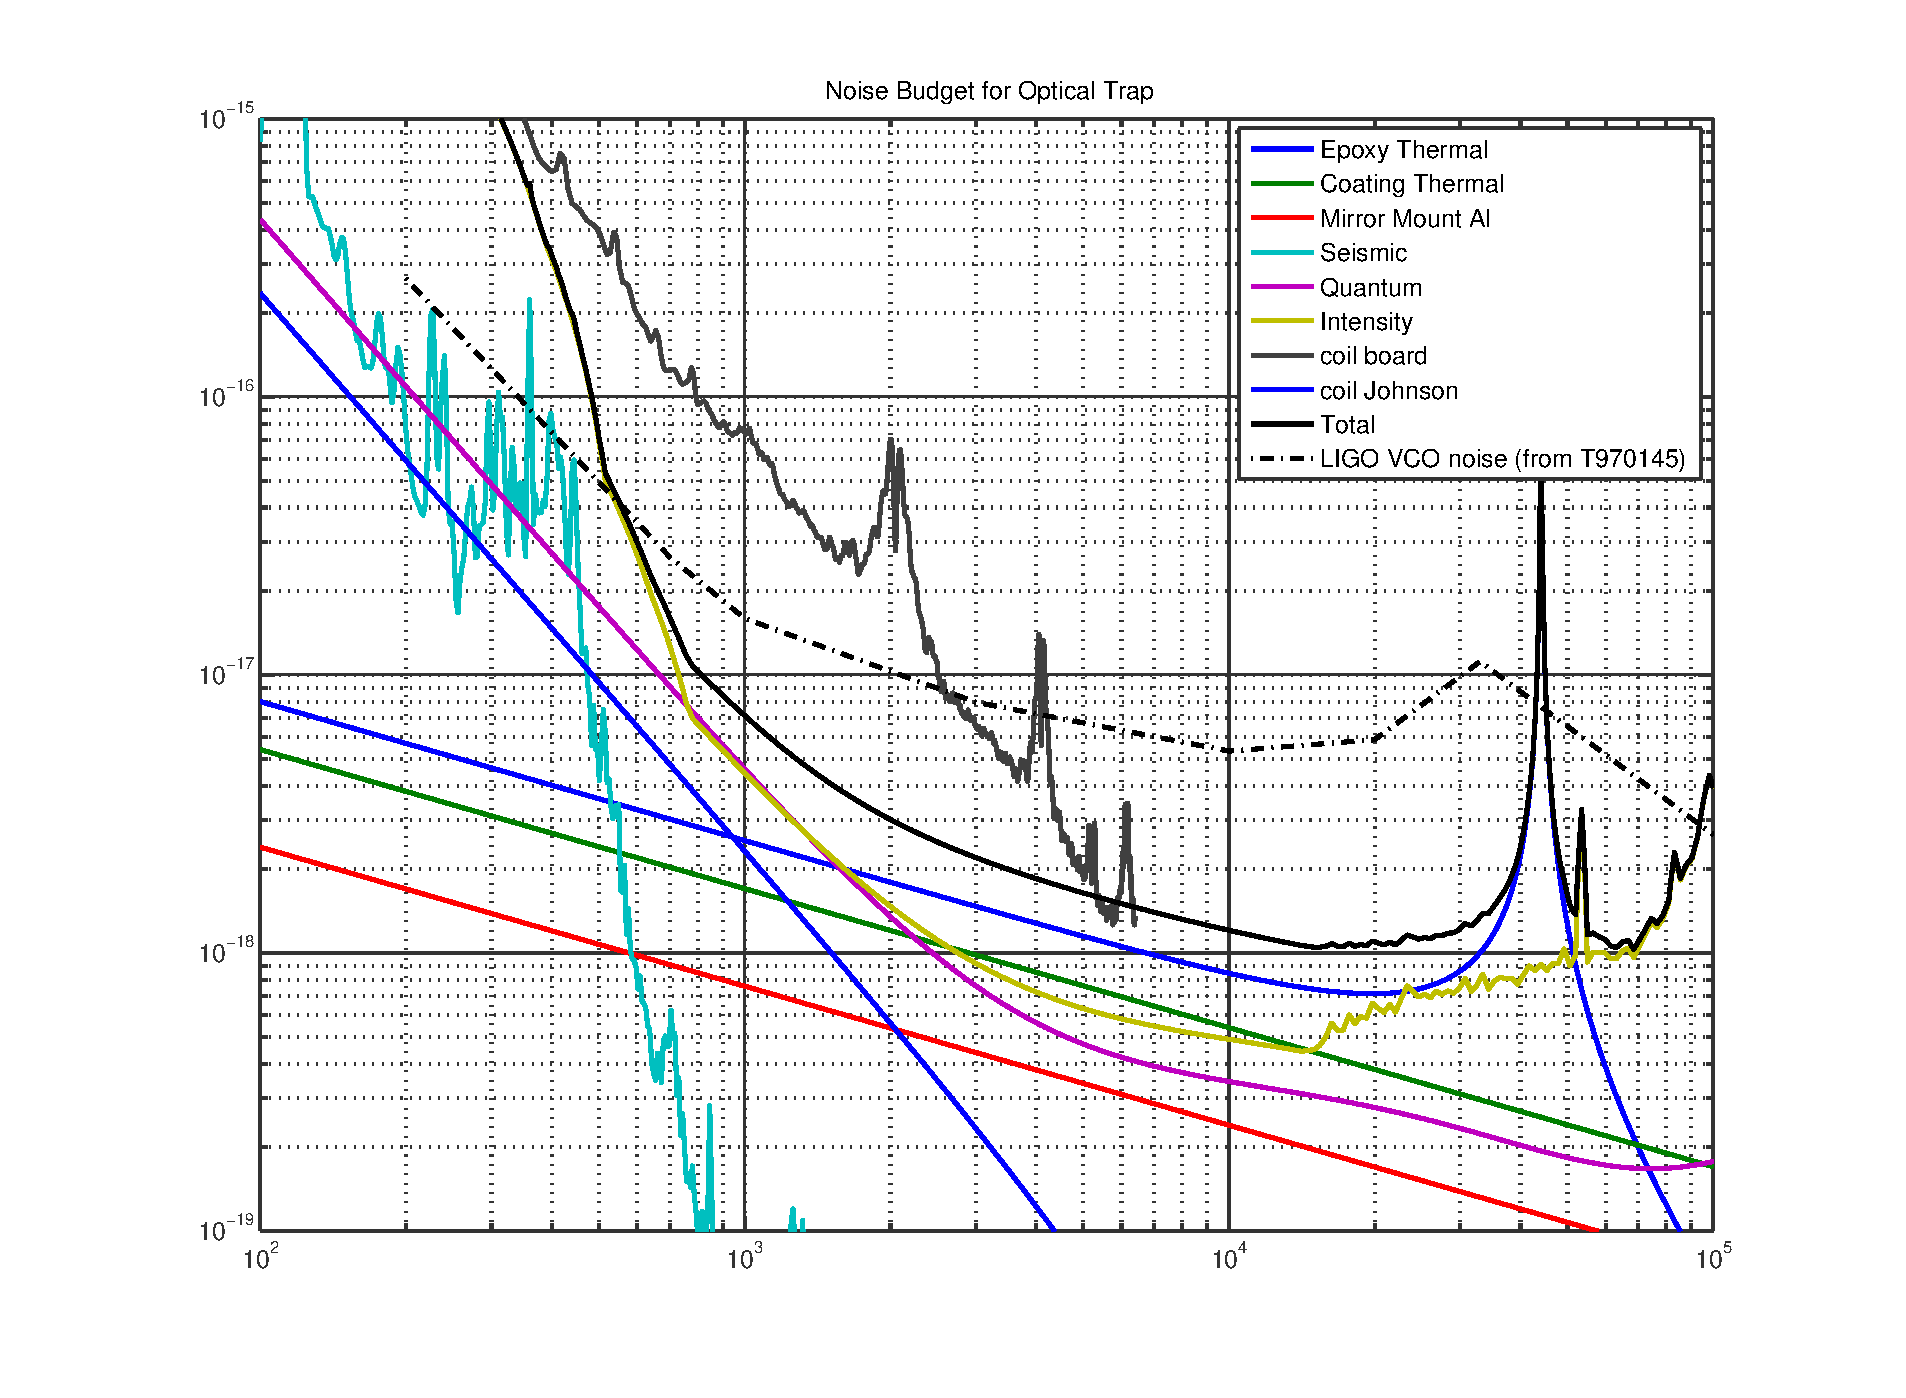
\includegraphics[width=15cm]{./figures/noise_budget.eps}
%	\caption[Noise Budget]{Noise budget}
%	\label{fig:noise_bud}
%\end{figure}
%
%\begin{figure}
%	\centering
%		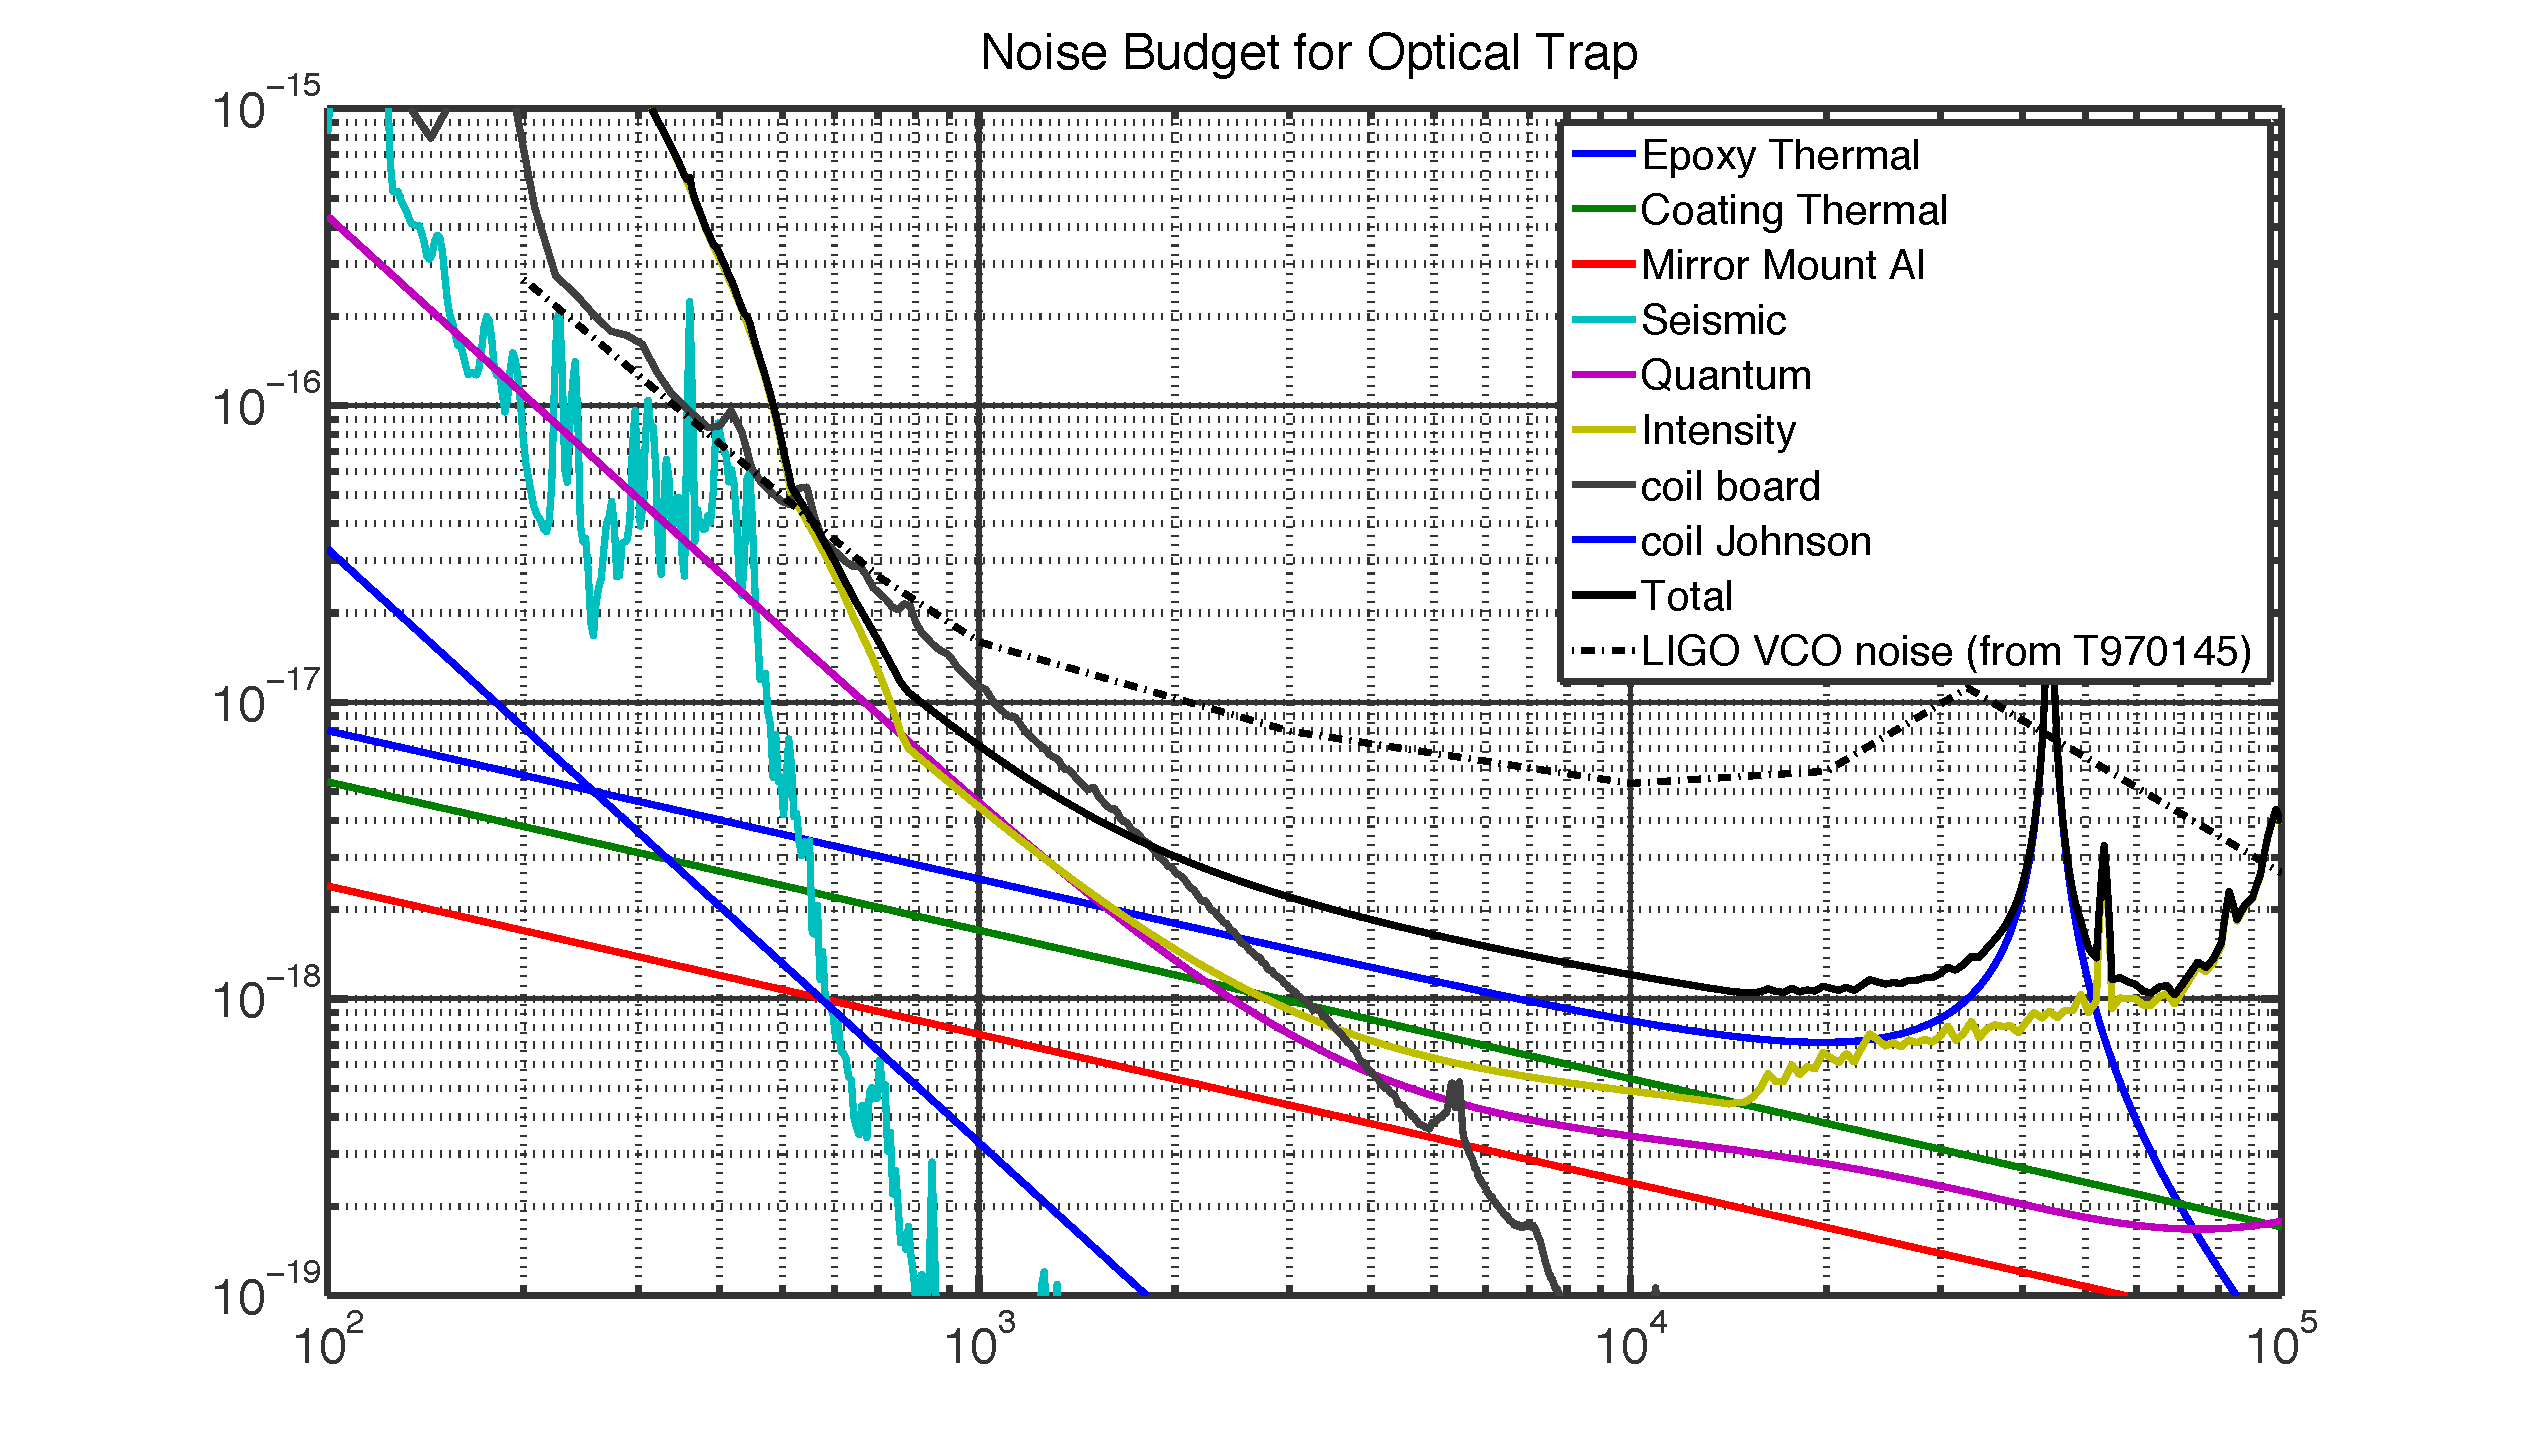
\includegraphics[width=15cm]{./figures/NoiseBudgetBoard.pdf}
%	\caption[Noise Budget Board]{Noise budget with coil driver board noise}
%	\label{fig:noise_bud_brd}
%\end{figure}
%
%\section{Vacuum Requirements for Optical Trap}
%
%It is desired to have an understanding of limits of vacuum gas constituents
%for the in-vacuum experiment.
%From the LIGO DCC we have a few documents that describe the process that went
%into understanding the problem for 2 4km long Fabry-Perot cavities.
%I will apply these techniques to a 10-30cm cavity.\\
%
%
%\subsection{LIGO Vacuum Requirements}
%
%The amplitude spectral density of the optical path length is given by,
%
%\begin{align*}
%\Delta L ( f ) = 4 \pi \left( \frac{2 L_0 p}{k T w_0 v_0} \right)^{1/2} a e^{- \pi f w_0 / v_0 }
%\end{align*} \\
%
%
%From *** the value for $4 \pi a \left( \frac{2}{k T w_0 L_0 v_0} \right)^{1/2} $ is $ 4.8 x 10^{-21} \left( \frac{R_x}{R_{H_2}} \right) $. Where $L_0 = 4000 \mathrm{m} $ and $ w_0 = 0.06 \mathrm{m} $. \\
%
%For our purposes (single arm cavity) we will lose a factor of $ \sqrt{2} $. \\
%
%We end up with a formula for amplitude spectral density in a one-arm cavity that is:
%
%\begin{align*}
%\Delta L ( f ) = 4 \pi \left( 5.3 \mathrm{x} 10^{-20} \right) \left(  \frac{R_x}{R_{H_2}} \right) \sqrt{\frac{ L_0 p}{ w_0 } } e^{- \pi f w_0 / v_0 }
%\end{align*} \\
%
%\subsection{Optical Trap}
%
%Now, we insert parameters for the cavity. For the first look, I use the parameters defined in the project description: 0.3m cavity length, 0.2m radius of curvature for each mirror.
%\todo{something},
%
%If we operate at a pressure of 1e-6 Torr, no constituent gas can be greater than this. The following plot is of constituent gases at this pressure.
%
%\begin{figure}
%	\centering
%		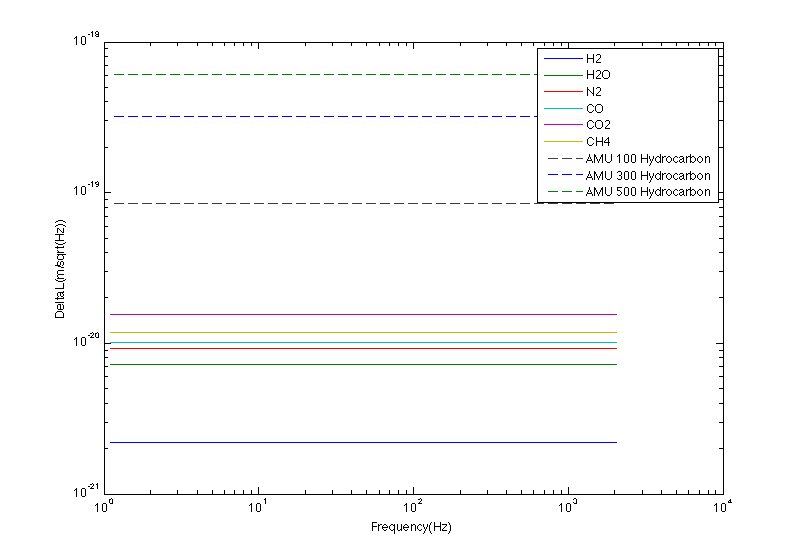
\includegraphics[width=15cm]{./figures/trapgasnoise_1.png}
%	\caption[Gas Noise Comparison]{Gas Noise for 1e-6 Torr}
%	\label{fig:gas_noise1}
%\end{figure}
%
%If we have a residual gas analyzer that detects a minimum partial pressure of 5e-11 Torr:
%
%\begin{figure}
%	\centering
%		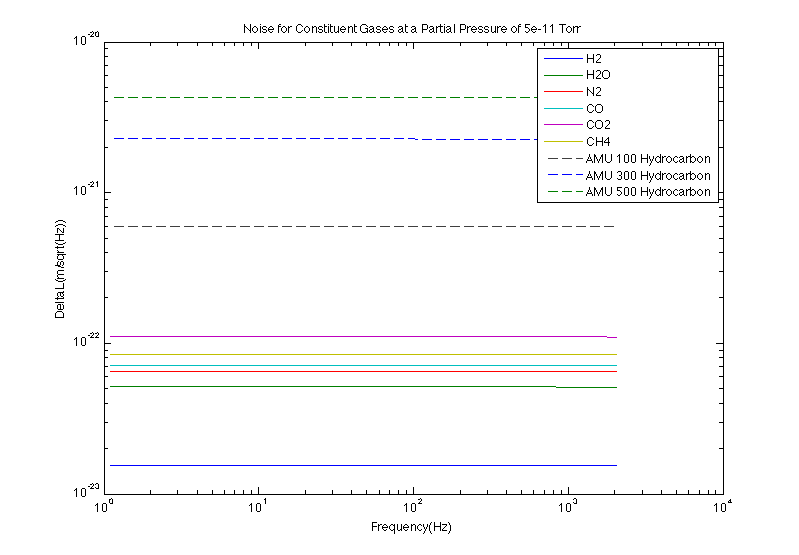
\includegraphics[width=15cm]{./figures/trapgasnoise_2.png}
%	\caption[Gas Noise Comparison]{Gas Noise for 5e-11 Torr}
%	\label{fig:gas_noise2}
%\end{figure}

%\section{Epoxy Thermal Noise}
%
%Brownian thermal noise estimates for epoxy joints are gotten from basic application of the fluctuation-dissipation theorem. The form that we start with is,
%\begin{align*}
%S_{x^2}(f) = \frac{4 k_B T}{\omega^2} \Re(Z^{-1}), 
%\end{align*}
%where $Z$ is the impedance, $F / v$. The force equation that we use is of the form,
%\begin{align*}
%F_{\mathrm{ext}} = m \ddot{x} + k x,
%\text{where k is a complex number}, (1 + i \phi)
%\end{align*}
%
%\section{Derivation}
%
%\begin{align*}
%d_n = d(t-\tau_n)
%\end{align*} \\
%
%\begin{align*}
%d_n = d \left( t - \frac{(2n -1)}{c} L_0 - d_1 - \sum_{l=2}^{n} 2 d_l \right)
%\end{align*} \\

